\documentclass[18pt,oneside,a4paper, titlepage]{article}

\usepackage[hidelinks]{hyperref}
\usepackage[pdftex]{graphicx}

\begin{document}
\title{\textbf{AOS project}\\ A.Y. 2015/2016\\
	Politecnico di Milano}	
\author{Barlocco Mattia, matr. 873801\\Belotti Nicola, matr. 793419\\Colombo Andrea, matr. 853381}
\date{September, 2016}
\maketitle

\newpage
\tableofcontents

\newpage
\section{Introduction}
	The goal of this project is to recognize which button of a remote control is pushed by using the BPW34 photodiode and the stm32f407. This board has a Analogic to Digital Converter (ADC) built-in that converts the anologic signal received from the BPW to a digital signal. This board operating system is Miosix.
	\begin{figure}[h]
		\centering
		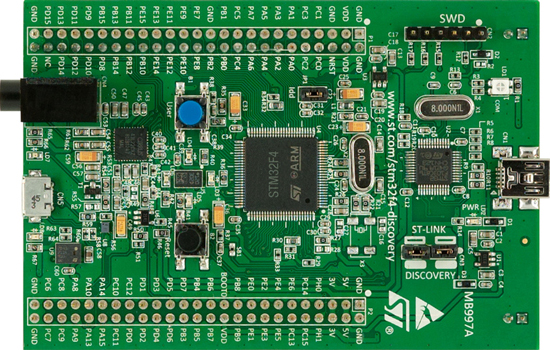
\includegraphics[scale=0.6]{board.jpg}%
	\end{figure}
\newpage
\section{BPW34}
	\begin{figure}[h]
		\centering
		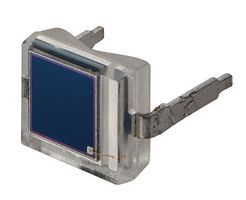
\includegraphics[scale=0.3]{fotodiodo.jpg}
	\end{figure}
	The BPW34 is a photodiode that is sensitive to visible and infrared radiation. Its carateristics are the following:
	\begin{itemize}
		\item It is sensitive at most 34KHz
		\item Fast response times
		\item Angle of half sensitivity: = ± 65°
		\item High photo sensitivity
		\item Suitable for visible and near infrared radiation
	\end{itemize}
	
For any other information on this photodiode visit: http://www.vishay.com/docs/81521/bpw34.pdf
\newpage
\section{How it works}
	\subsection{Board configuration}
	Used pins are the following:
		\begin{itemize}
			\item GND: BPW34 black wire 
			\item GND: FTDI black wire
			\item PC1: BPW34 red wire 
			\item PB10:FTDI yellow wire 
			\item PB11:FTDI orange wire  
			\item VDD: FTDI black wire 
		\end{itemize}

\newpage
\section{Used Software}
\begin{itemize}
	\item QSTlink2: used to program the board.
	\item Github: to save every code changes  online.
	\item Latex: to write this document.
	\item Notepad++: to write code.
	\item Miosix Toolchain: to compile the project
	\item ArduinoIDE: serial Arduino monitor 

\end{itemize}

\end{document}